% !TEX root = ../thesis.tex
\renewcommand\appendixtocname{Anhänge}
\renewcommand\appendixpagename{Anhänge}
\begin{appendices}

\chapter{Weitere Abbildungen}

\begin{figure}[H]
\centering
\begin{tabular}{cc}
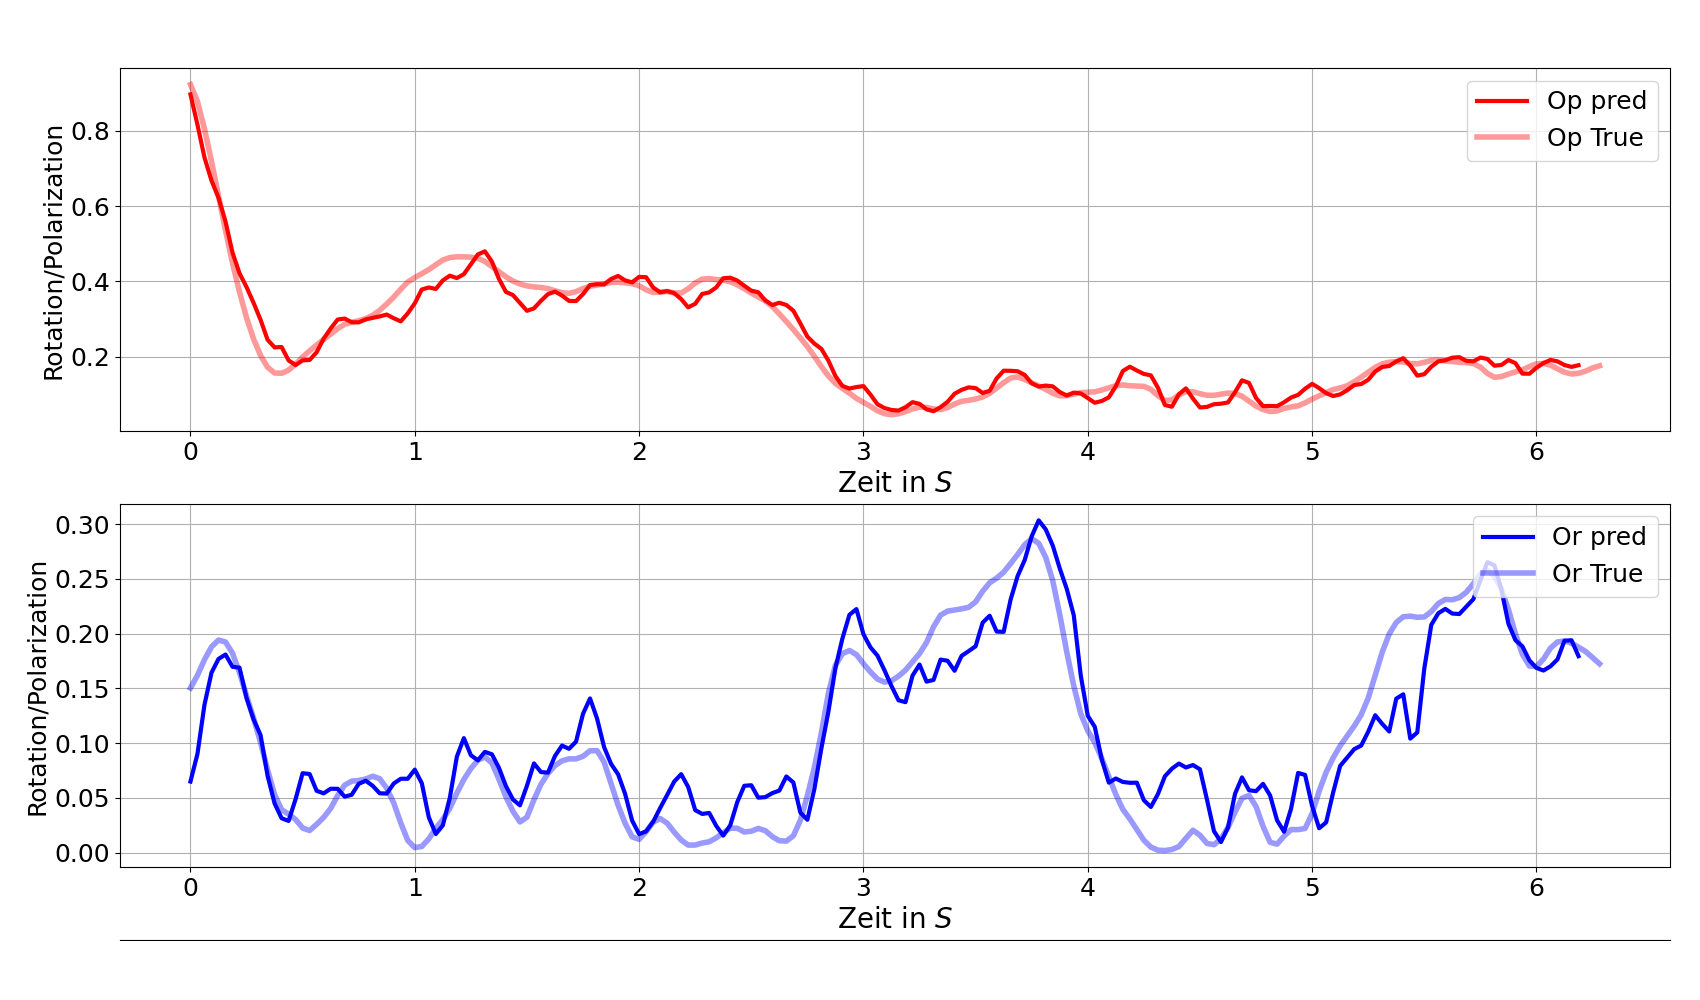
\includegraphics[width=1.0\textwidth]{figures/Anhang/Boids_random_False.png} 
\end{tabular}
\caption{Zustände Boids für konstante Parameter }
\end{figure}

\begin{figure}[H]
\centering
\begin{tabular}{cc}
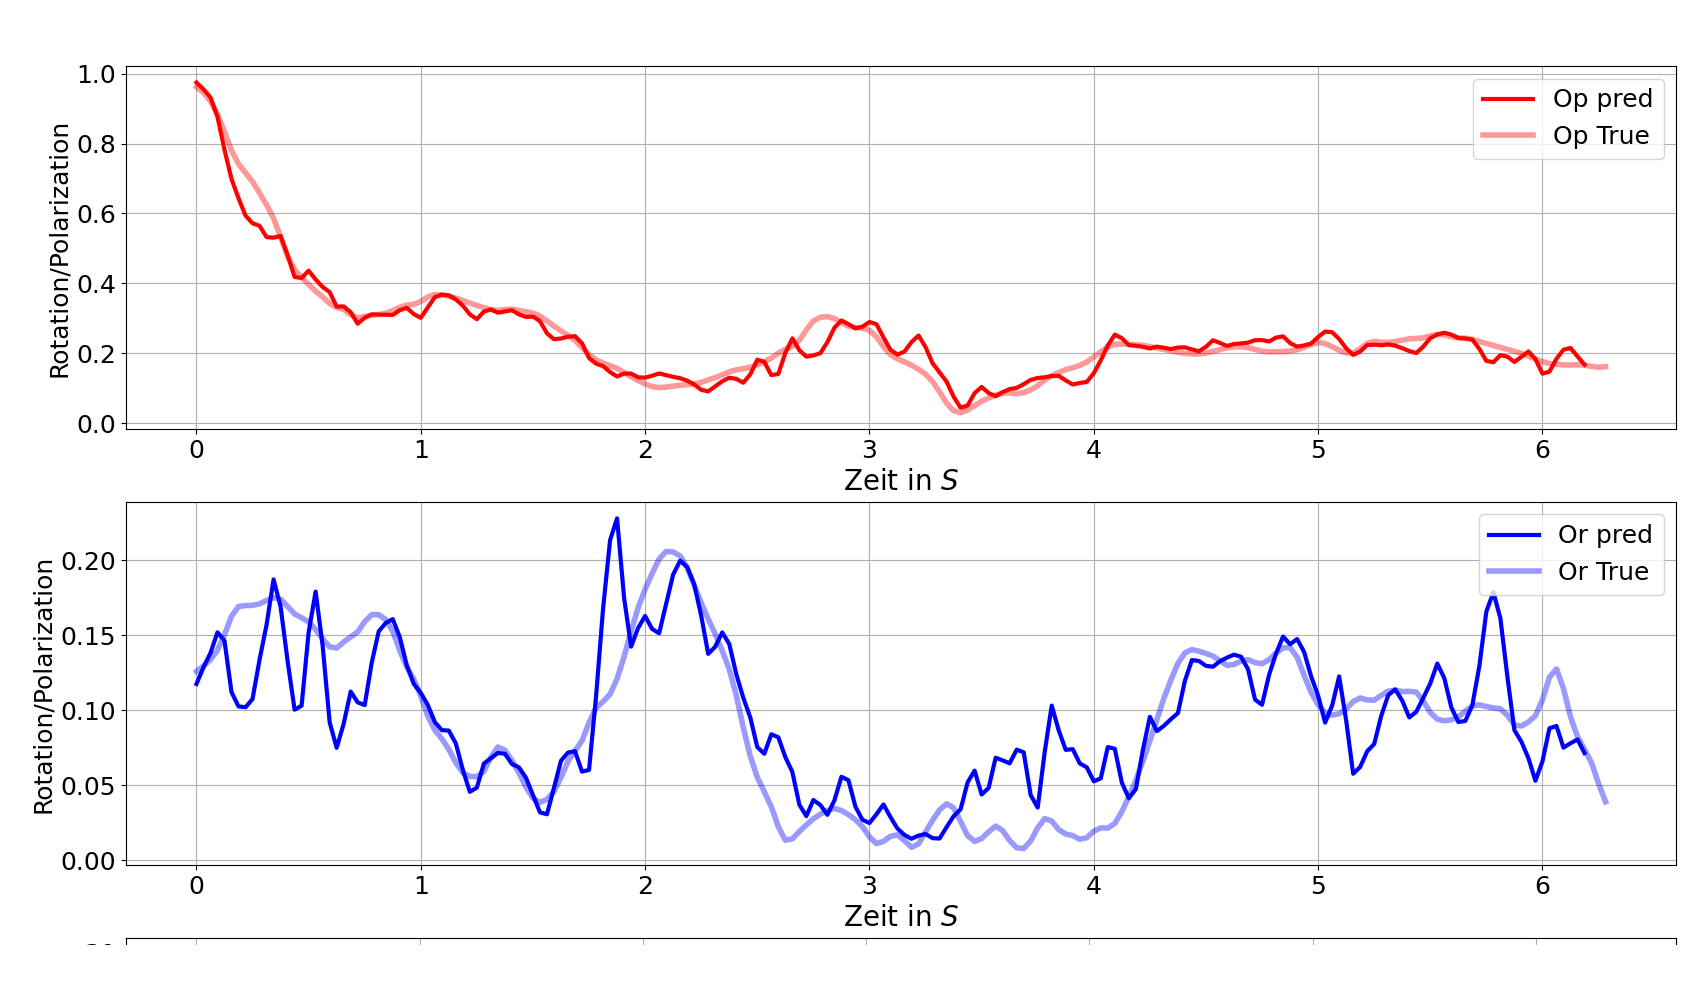
\includegraphics[width=1.0\textwidth]{figures/Anhang/Boids_random_True.png} 
\end{tabular}
\caption{Zustände Boids für variable Parameter }
\end{figure}

\begin{figure}[H]
\centering
\begin{tabular}{cc}
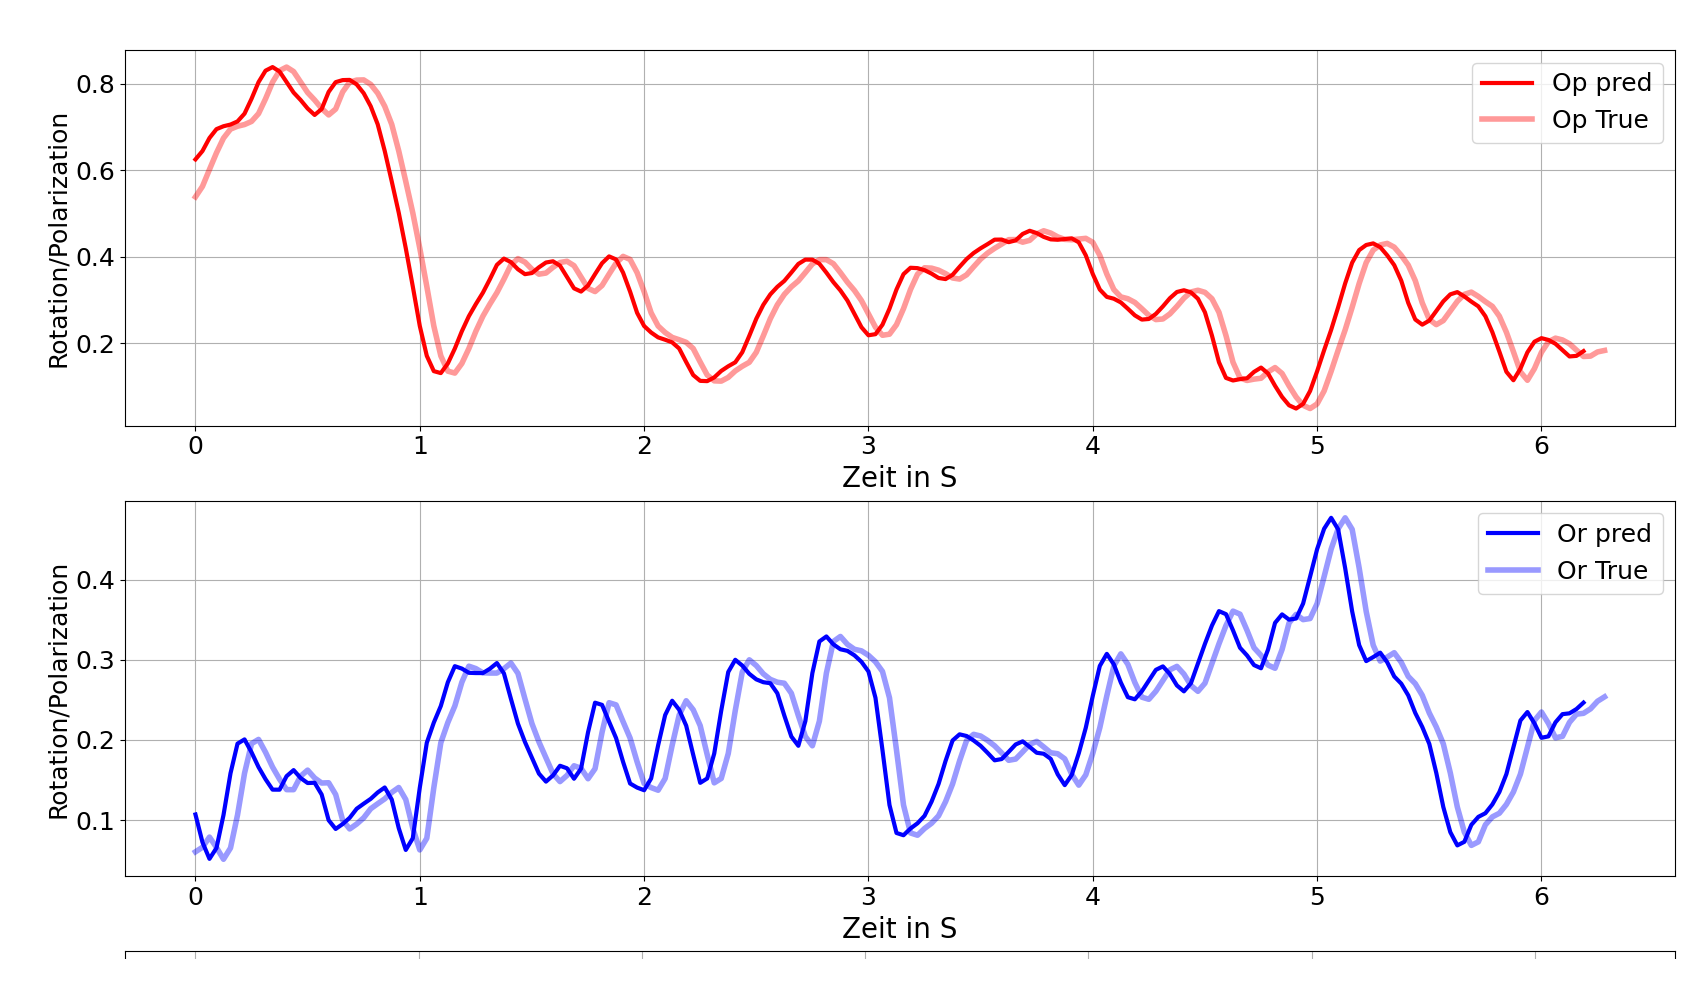
\includegraphics[width=1.0\textwidth]{figures/Anhang/PWD_random_False.png} 
\end{tabular}
\caption{Zustände eigenes Modell für konstante Parameter }
\end{figure}

\begin{figure}[H]
\centering
\begin{tabular}{cc}
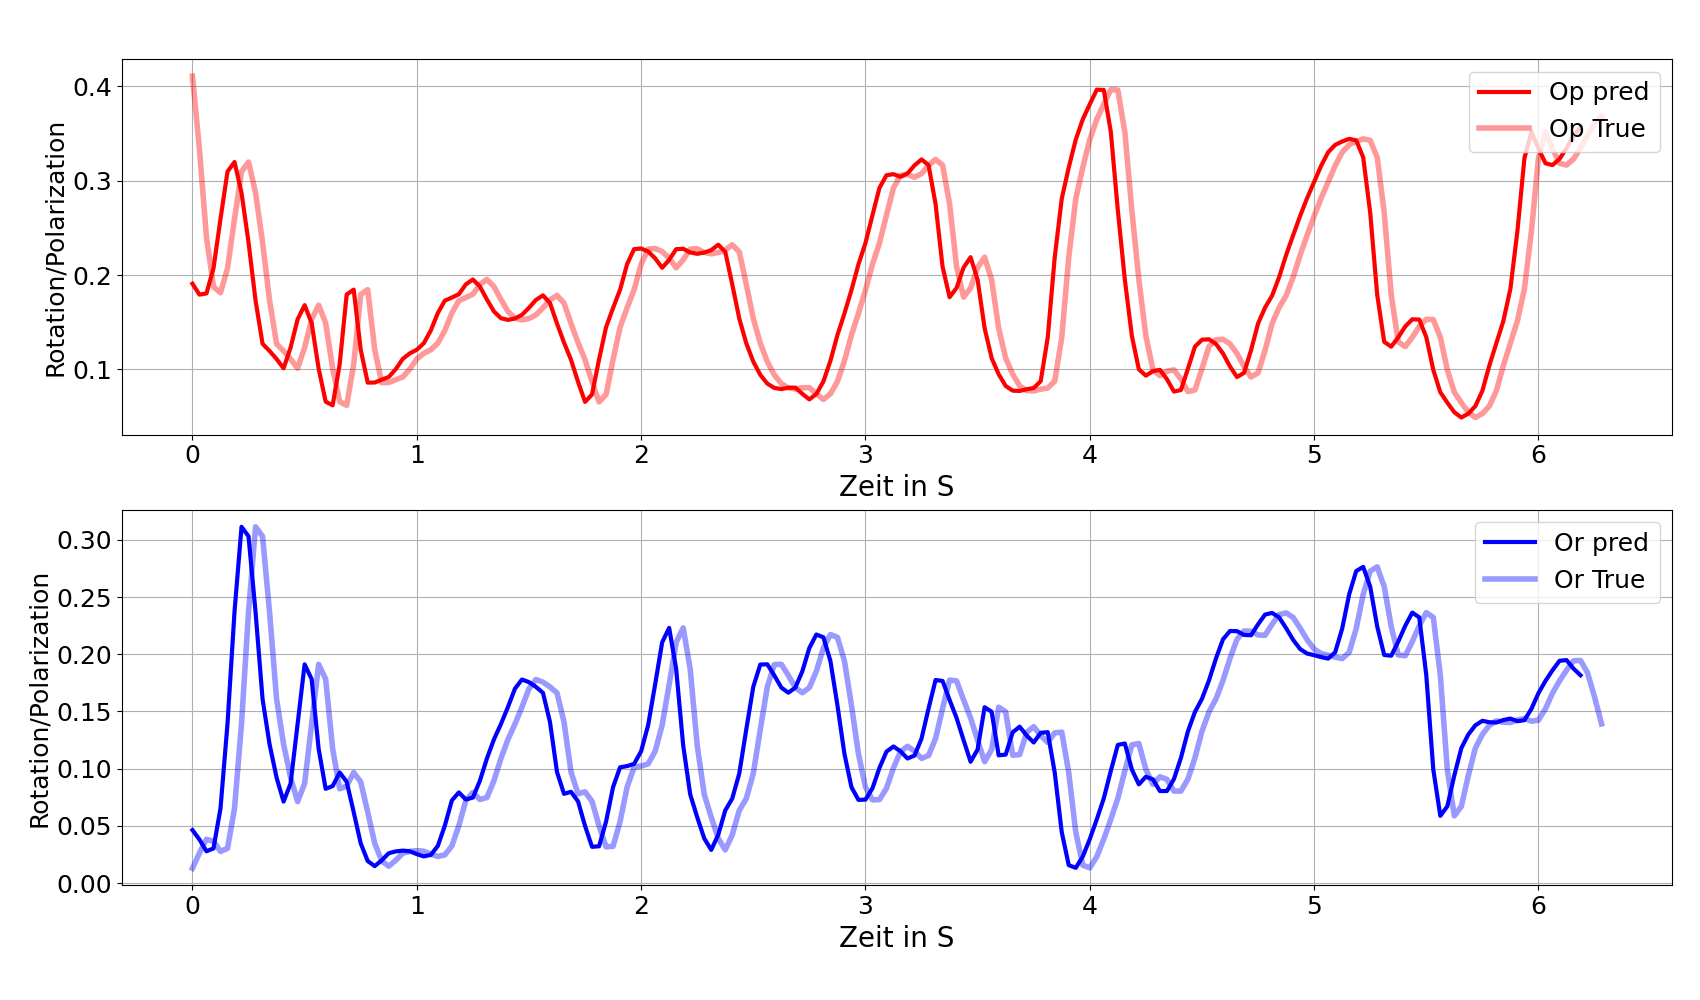
\includegraphics[width=1.0\textwidth]{figures/Anhang/PWD_random_True.png} 
\end{tabular}
\caption{Zustände eigenes Modell für variable Parameter }
\end{figure}

\begin{figure}[H]
\centering
\begin{tabular}{cc}
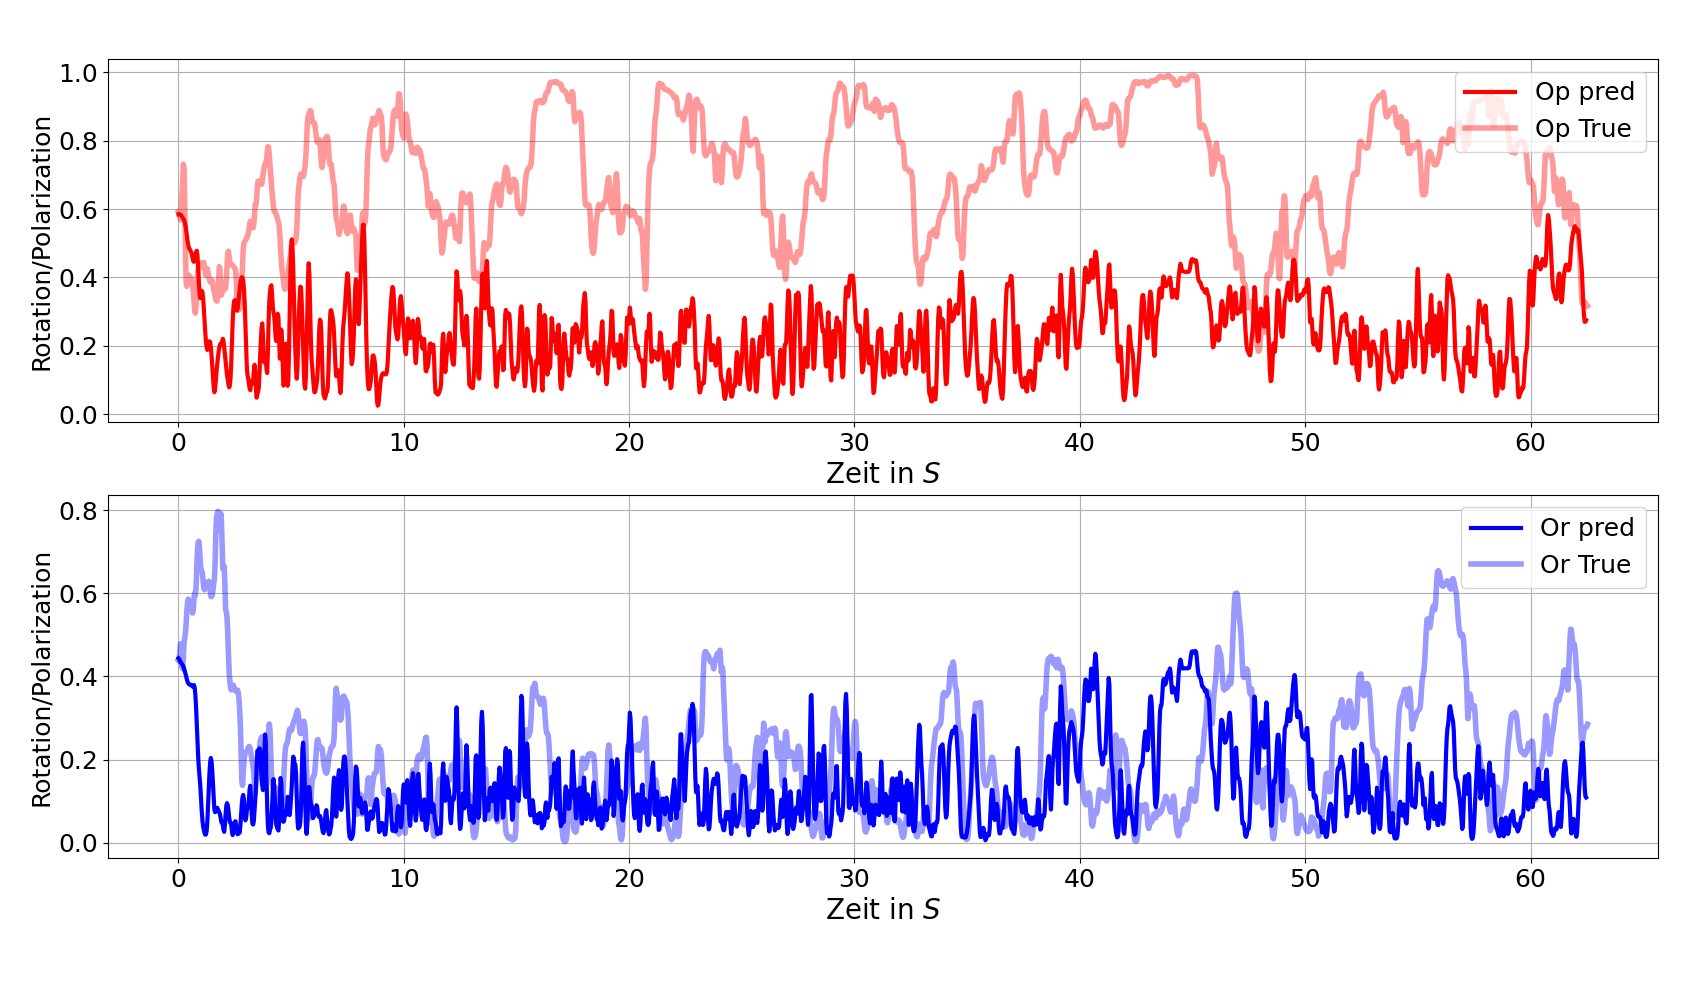
\includegraphics[width=1.0\textwidth]{figures/Anhang/Boids_10.png} 
\end{tabular}
\caption{Zustände Boids der Schwarmgröße 10 }
\end{figure}

\begin{figure}[H]
\centering
\begin{tabular}{cc}
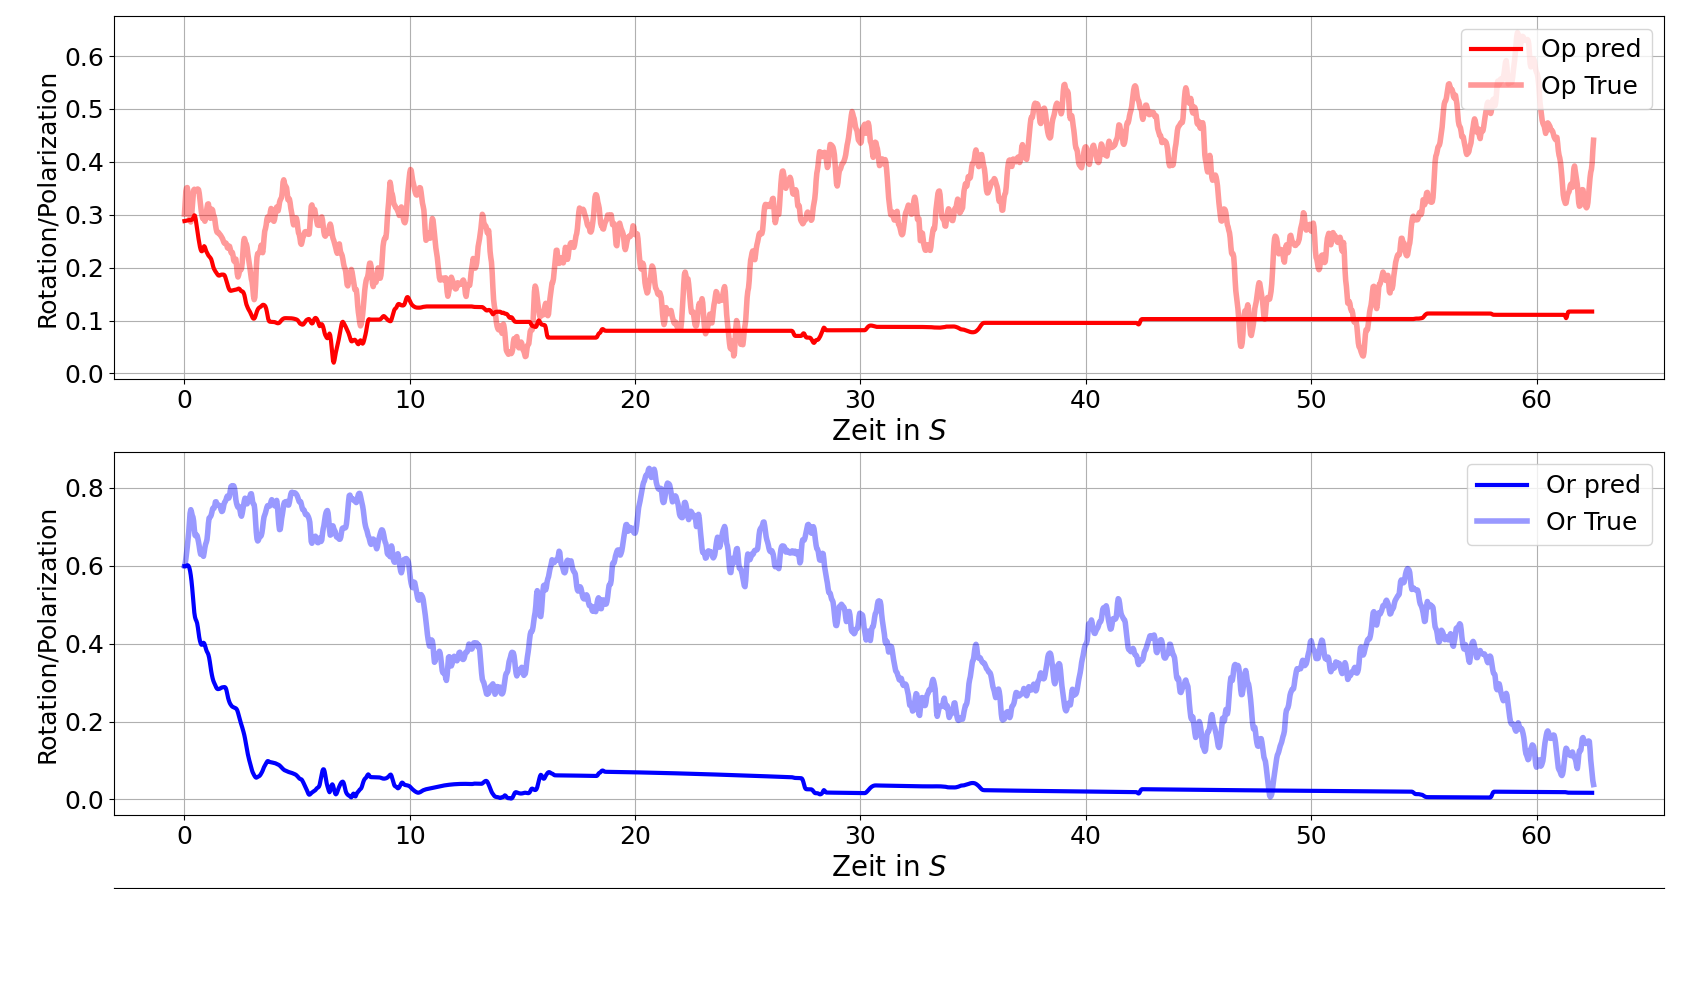
\includegraphics[width=1.0\textwidth]{figures/Anhang/Boids_60.png} 
\end{tabular}
\caption{Zustände Boids der Schwarmgröße 60 }
\end{figure}

\begin{figure}[H]
\centering
\begin{tabular}{cc}
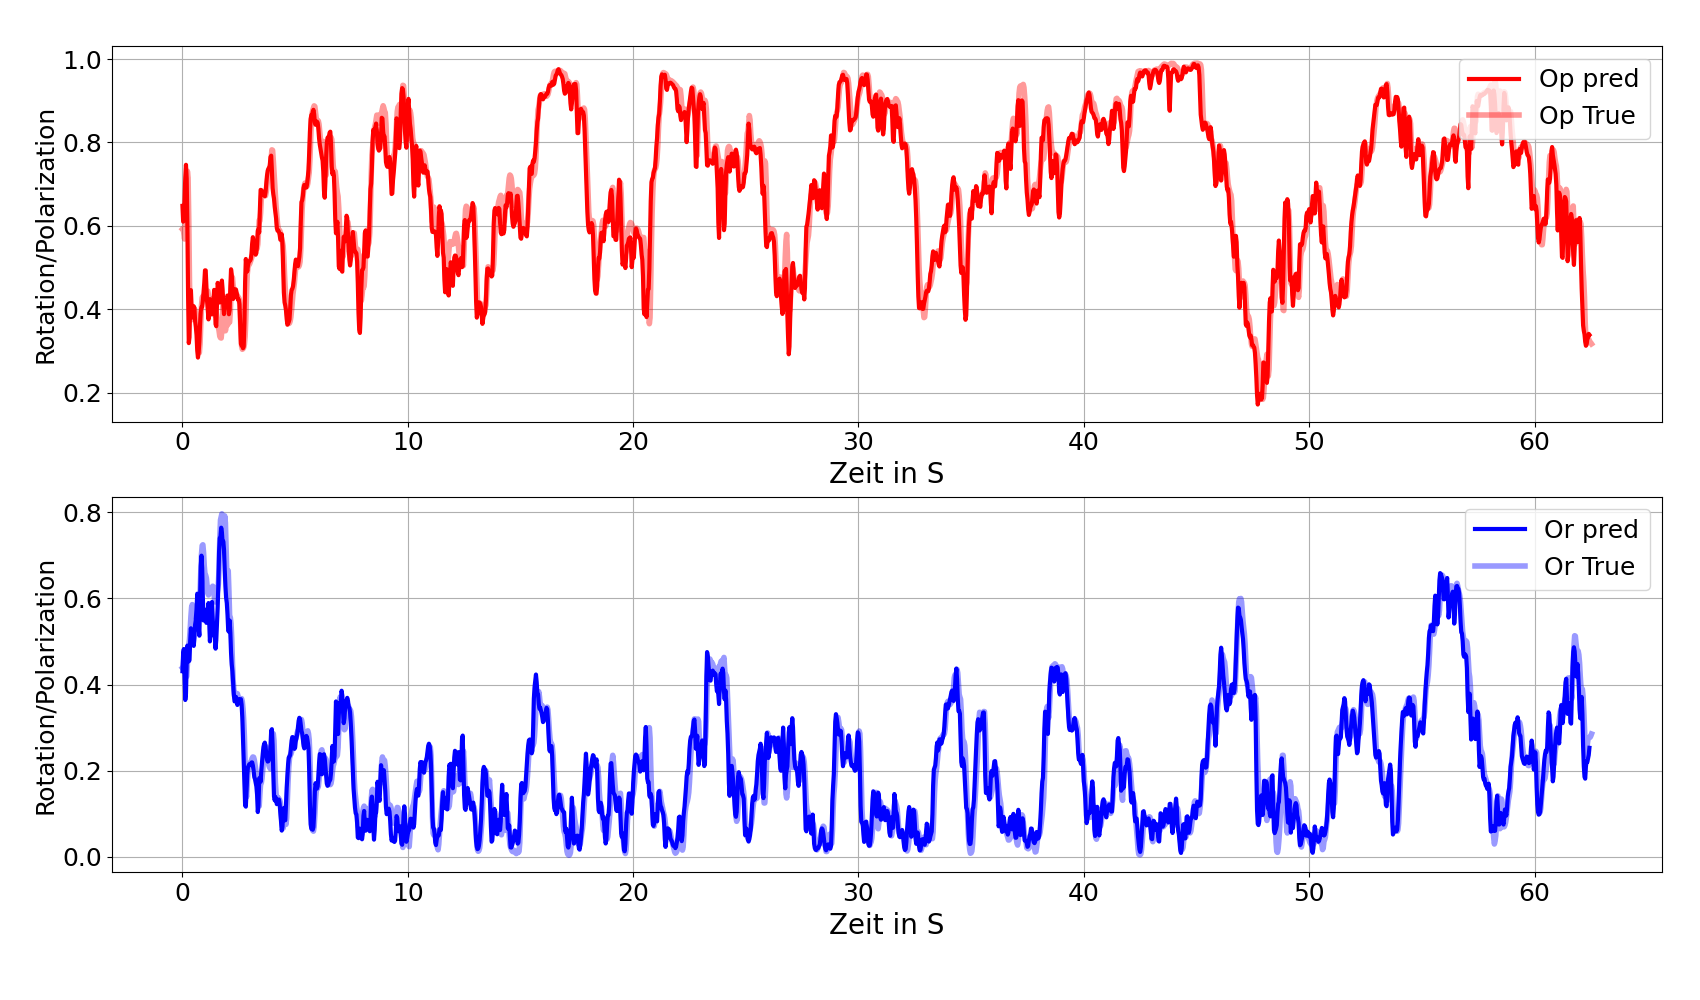
\includegraphics[width=1.0\textwidth]{figures/Anhang/PWD_10.png} 
\end{tabular}
\caption{Zustände eigenes Modell der Schwarmgröße 10 }
\end{figure}

\begin{figure}[H]
\centering
\begin{tabular}{cc}
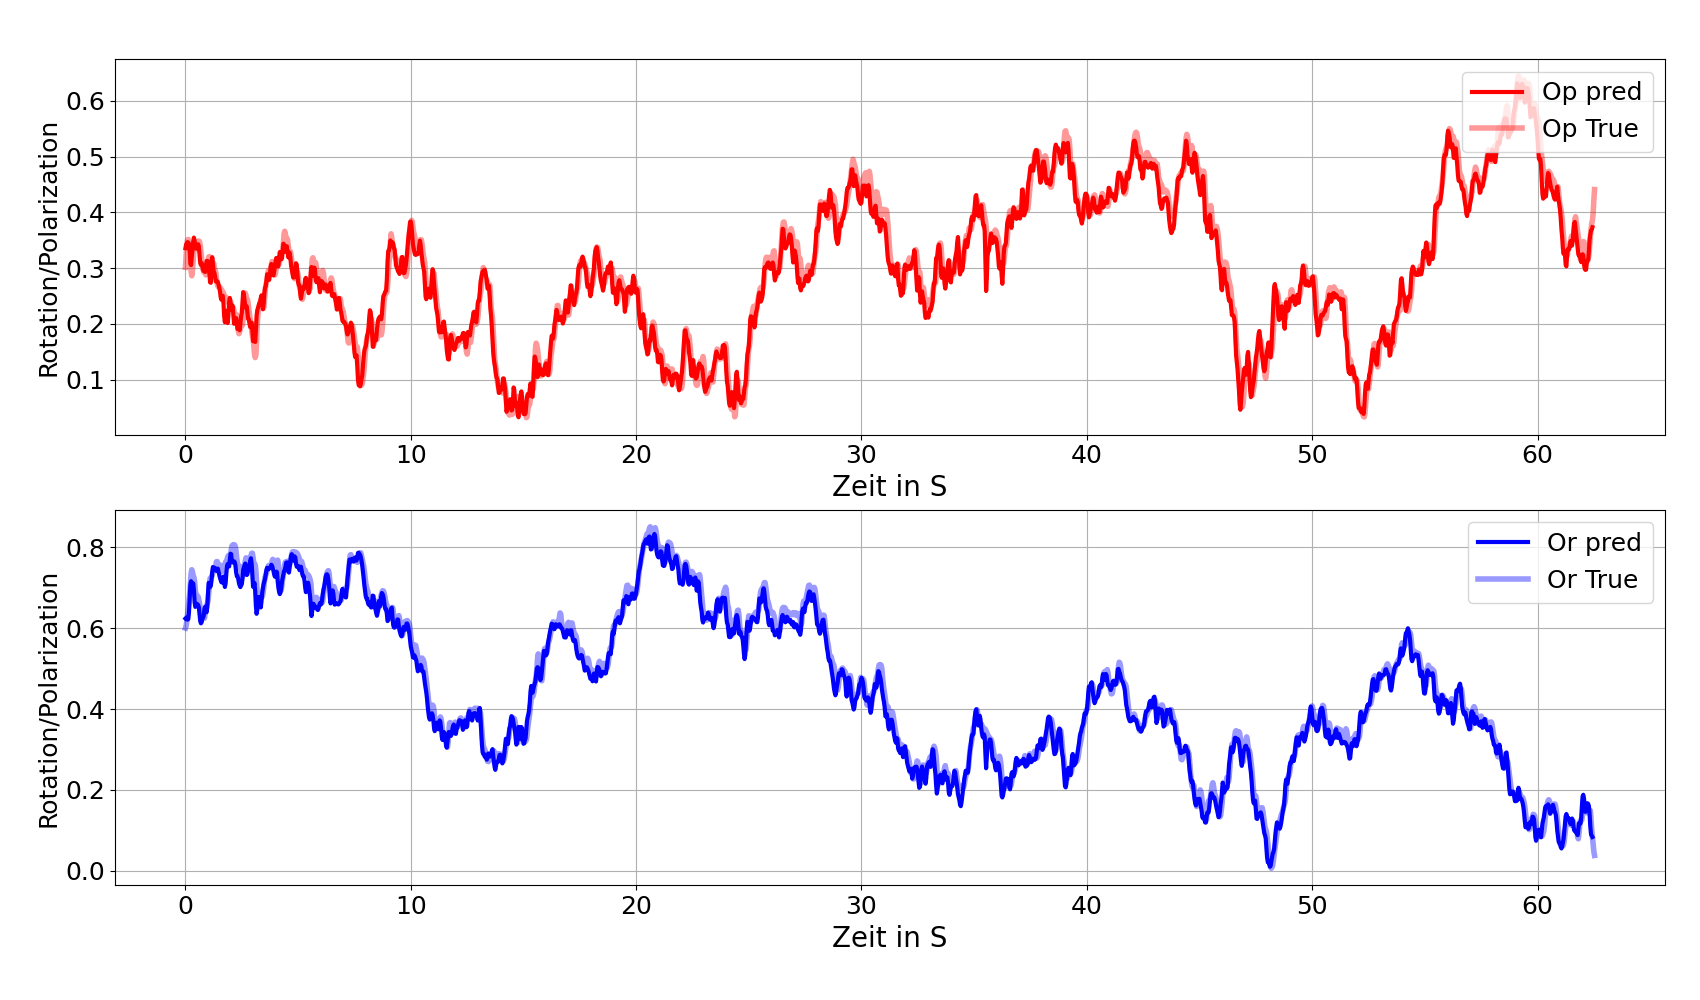
\includegraphics[width=1.0\textwidth]{figures/Anhang/PWD_60.png} 
\end{tabular}
\caption{Zustände eigenes Modell der Schwarmgröße 60 }
\end{figure}

\end{appendices}